\documentclass[thesis.tex]{subfiles}

\begin{document}
\ifSubfilesClassLoaded{

% \section{Definitions}
% \todo[inline]{These will be defined in the introductory chapters, but are here so that this draft is understandable}
% \begin{itemize}
% \item
%   We assume that, for all episodes $i$, $D_i$ is iid and independent
%   of the time of the infection. Define the survival function
%   $\prob(D_i \geq t \mid B_{j} = b, \vec{\theta}) = \prob(D_i \geq t \mid \vec{\theta}) = S_{\vec{\theta}}(t)$,
%   where $\vec{\theta}$ are the parameters controlling the survival
%   distribution (the discussion in this document is valid regardless of
%   the model specified for $S_{\vec{\theta}}$ and hence we consider $\vec{\theta}$
%   as an arbitrary vector of parameters).
% \item
%   The beginning of episode $i$ is known to occur in the interval
%   $[l_{j}^{(b)}, r_{j}^{(b)}]$, and similarly for the end of the infection
%   in $[l_{j}^{(e)}, r_{j}^{(e)}]$.
% \end{itemize}

\setcounter{chapter}{4}
}

\chapter{Estimating duration with infrequent testing} \label{perf-test}

When estimating incidence from prevalence, the mean duration, not its median, is the most important feature of the duration distribution~\autocite{freemanPrevalence}.
Duration distributions tend to be right-skewed.
Therefore, estimates of the mean would be sensitive to the tail of the duration distribution.

In \cref{E-ATACCC} I estimated the duration distribution from the ATACCC dataset.
However, this study had a small sample size and only 20 days of follow-up, which prevented accurate estimation of the tail.
Therefore, model assumptions drive the estimated size of the tail.

The CIS samples individuals less frequently, but has a large sample size (\numprint{4800} detected infection episodes) and up to years of follow-up.
Therefore, it is suitable for estimating the tail of the duration distribution.
In this chapter, I develop a method to estimate the duration distribution using CIS data, assuming the test ??? has perfect sensitivity and specificity, {\it i.e.} there are no false negatives or positives.
Formally, I aim to estimate the survival function $S(t)$ defined in \cref{inc-prev:sec:definitions}.

In \cref{perf-test:sec:problem}, I describe the challenges analysing the data presents.
This motivates using a survival analysis framework which I introduce in \cref{perf-test:sec:surv-analysis}, before deriving the statistical model for the CIS setting in \cref{perf-test:sec:model}.
In \cref{perf-test:sec:parameters-priors}, I consider how to parameterize the survival function and choose its priors, including vague and smoothing priors as well as a prior constructed to include the information from \cref{E-ATACCC}.
I evaluate the model and priors using a simulation study (\cref{perf-test:sec:simulation-study}), showing that they perform well.
Finally, I discuss the results in \cref{perf-test:sec:discussion}.

\section{Problem description} \label{perf-test:sec:problem}

In the CIS, individuals are tested infrequently, either weekly or monthly (see \cref{E-intro:sec:cis}), complicating the data in two ways.
First, infection episodes can go undetected.
Second, the infection episode start and end times are known imprecisely.
I explain these issues below, and devote the rest of the chapter to the development of a method to tackle  them.

\subsection{Undetected infections} \label{perf-test:sec:undetected}

The first complication in the analysis is that infection episodes can be undetected.
Undetected infection episodes are episodes with no associated positive tests.
Therefore, there is no information directly observed about the episode; even the number that occur is latent.
They occur when an episode starts and ends between tests (see \cref{perf-test:fig:truncation}).
Undetected episodes are important because they are, on average, shorter than detected episodes; therefore, neglecting them would lead to a biased estimate of the survival distribution.
To see why this is the case, consider the infection episode in figure \cref{perf-test:fig:truncation}.
Here two individuals are shown, with identical data collected for each of them (a series of negative
tests).
The fist individual was never infected whereas the second individual was; but their infection episode was undetected.
The undetected infection episode begins at time 33 and has a 10-day duration.
The individual would have been detected at their next test if their duration had instead been 24 days or more.
The gap between tests in the CIS (up to 28 days, see \cref{E-intro:sec:cis}) is longer than the duration of most infections (median 16 days, see \cref{E-ATACCC:sec:results}).
Therefore, it is likely that many infection in the CIS cohort were undetected.
This is because the interval between tests in the same individual (up to 28 days, see \cref{E-intro:sec:cis}) is longer than most infections (median 16 days, see \cref{E-ATACCC:sec:results}).
\begin{figure}
  \makebox[\textwidth][c]{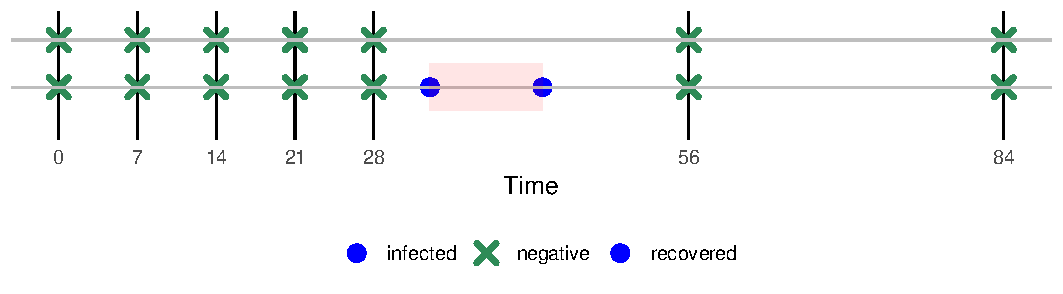
\includegraphics[width=\textwidth]{cis-perfect-testing/truncation}}
  \caption[Undetected episodes in CIS data]{Graphical illustration of an undetected infection episode, represented by the shaded area. \label{perf-test:fig:truncation}}
\end{figure}

\subsection{Unobserved times for each episode's beginning and end} \label{perf-test:sec:interval-censoring}

The second complication is that the beginning and end times of detected infection episodes are latent.
Recall, from \cref{E-biology-data:sec:cis-episodes}, that the time episode $j$ starts, $b_j$, is only known to lie in the interval $[l_j^{(b)}, r_j^{(b)}]$ where $l_j^{(b)}$ is the day after the negative test prior to the start of episode $j$ and $r_j^{(b)}$ is the first positive test in episode $j$.
Similarly, for the end of the infection episode, $e_j \in [l_j^{(e)}, r_j^{(e)}]$.
\Cref{perf-test:fig:double-interval-censor} shows this issue graphically.
\begin{figure}
  \makebox[\textwidth][c]{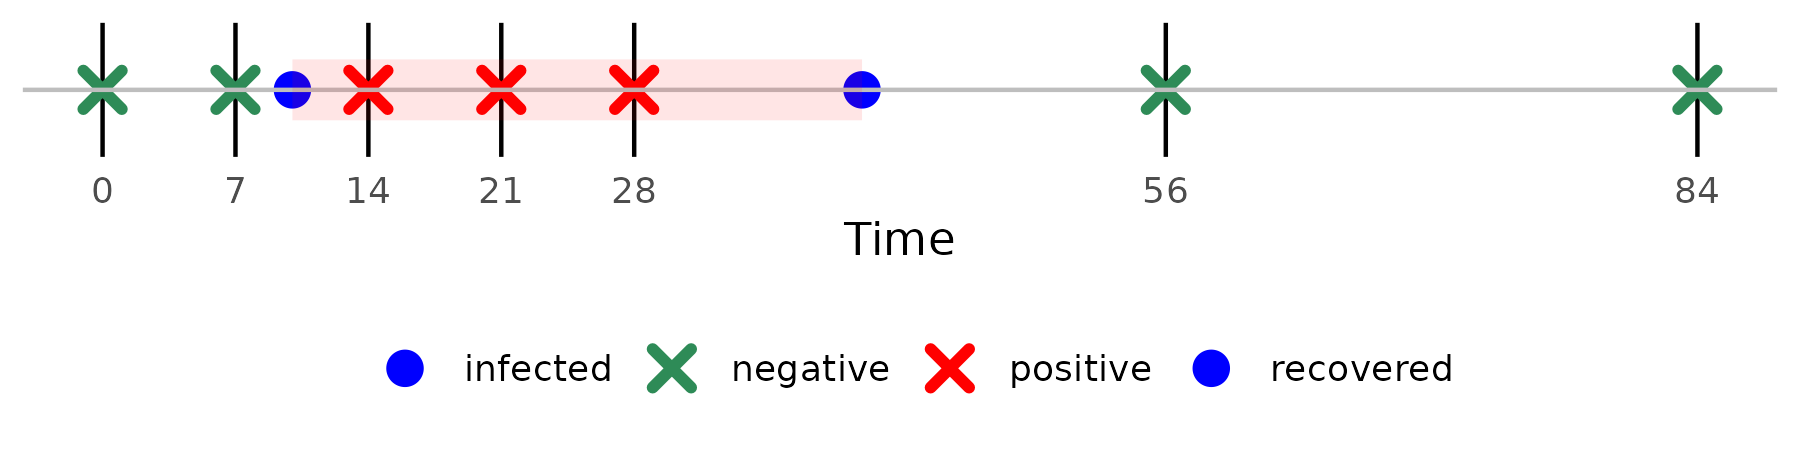
\includegraphics[width=\textwidth]{cis-perfect-testing/double-interval-censor}}
  \caption[Double-interval censoring in CIS data]{%
        The beginning and end of each episode observed in the CIS data is only known up to an interval.
        Demonstrated here by a participant who is recorded negative at time 7 and positive at time 14, bounding the start of the episode; similarly, changing from positive at time 28 to negative at time 56 bounds the end of the episode.
    }
    \label{perf-test:fig:double-interval-censor}
\end{figure}

\section{Survival analysis} \label{perf-test:sec:surv-analysis}

In survival analysis, the interest is in estimating the distribution of the interval between an \emph{initiating event} and a \emph{terminating event}.
In the current context, the initiating event is the episode's start; the terminating event is the episode's end.
I start by introducing the relevant, standard concepts in survival analysis; a wide range of texts cover them including \textcite[chapter 1]{bogaertsSurvival}.

A common issue is that the initiating and/or terminating events are not known exactly.
This is known as the event being \emph{censored}.
An event is \emph{left censored} if it is known to have occurred before a certain time.
An event is \emph{right censored} if it is known to have occurred after a certain time.
An event is \emph{interval censored} if it is known to have occurred within an interval.
If both the initiating and terminating event are interval censored, the data are \emph{doubly interval censored}.
To handle doubly interval censored data, the times need to be jointly modelled~\autocite[and references therein]{liSemiparametric}.

Another important concepts typical of survival data is truncation, which refers to ...?
Sometimes, only intervals satisfying some property are recorded.
In this case, data are \emph{truncated}.
\emph{Left truncation} is when only events lasting longer than a minimum amount of time are observed.
\emph{Right truncation} is when only events lasting shorter than a maximum amount of time are observed.
Without correcting for truncation, inference on the distribution of a duration will be biased.

In the CIS data, the initiating and terminating events are only bounded (see \cref{perf-test:sec:interval-censoring}).
Therefore, the data are doubly interval censored.

There is also undetected infections in the CIS (see \cref{perf-test:sec:undetected}).
However, the situation is subtly different from the standard truncation situation encountered in the literature.
In the standard situation, nothing is known about the unrecorded intervals.
But in CIS, individuals in which undetected infections occurred are enrolled in the study.
Therefore, we know the times that they were tested.
This provides information on how long their infections may have occurred.
I refer to these events as ``undetected'', rather than truncated, to emphasise this difference.

\Textcite{sunAnalysis,bogaertsSurvival} review methods for doubly interval censored data.
However, few studies look at data both doubly interval censored and with undetected (or truncated) events.
% This is especially true within the biostatistical literature on human diseases.
General theoretical frameworks, which include this case, have been developed~\autocite{turnbullEmpirical,dempsterMaximum}.
Yet only the special case where the terminating event is either uncensored or right censored has been applied in practice~\autocite[e.g.][]{sunEmpirical,bacchettiNonparametric,shenNonparametric}.
These studies base their inference on a likelihood contribution for each detected infection episode conditional on $b_j \in [l_j^{(b)}, r_j^{(b)}]$.

For this conditional likelihood to be valid, they assume this conditioning provides negligible information on the distribution of interest~\citePersonalComms{Nick Jewell}.
This assumption performs well in these settings, when the length of the intervals is fairly constant.
In particular, when the interval lengths are near-constant, $p(\text{episode $j$ detected} \mid b_j \in [l_j^{(b)}, r_j^{(b)}]) \approx p(\text{episode $j$ detected})$.
However, in the CIS (see \cref{E-intro:sec:cis}) the interval lengths change from one to four weeks.

Infection episodes in an individual's one-week testing period are over-represented in the detected infections.
This is because more frequent testing will detect a higher proportion of infections.
Therefore, for the average detected episode, $p(\text{episode $j$ detected} \mid b_j \in [l_j^{(b)}, r_j^{(b)}]) > p(\text{episode $j$ detected})$.
Therefore, conditioning on $b_j \in [l_j^{(b)}, r_j^{(b)}]$ is inappropriate.

Doubly interval censored and truncated data are common when assessing the survival time of bird and insect nests~\autocite{heiseyABCs}.
\textcite{heiseyModelling}, building on long-standing methodology~\autocite{dempsterMaximum,turnbullEmpirical}, develops a likelihood-based inference framework, allowing for arbitrary truncation patterns and double interval censoring.
They apply it to a situation where the visit times (possible detection times) are common to all the individuals, simplifying the likelihood.
I adapt this framework for CIS, when each individual has their own visit schedule (see section \cref{perf-test:sec:model}).

I use Bayesian inference for two reasons.
First, the frequentist properties (\eg consistency and convergence rate) of proposed estimators are poorly understood~\autocite{sunAnalysis,dengNonparametric}.
Second, a prior can include information from previous studies, such as from \cref{E-ATACCC}.
Alternatively, the prior can favour a smoothly changing hazard, which is biologically sensible, and can overcome issues caused by the undetected episodes ~\autocite{caoBias}.

Bayesian methods have been used for nest survival before~\autocite{heBayesiana,heBayesian,caoModeling} by augmenting the data with the unobserved times of infection.
The data augmentation approach creates a parameter for each detected infection.
This increases the dimensionality of the problem greatly, making it computationally infeasible with the large sample size of the CIS within the SRS.


\section{Modelling the duration}\label{perf-test:sec:model}

In this section, I develop a statistical model accounting for double interval censoring and undetected episodes.
In \cref{perf-test:sec:data-notation}, I introduce the data and notation, defining which quantities are observed and which are latent.
Then, in \cref{perf-test:sec:episode-types}, I apply the framework of \textcite{heiseyModelling} to classify possible episode beginning and end types into \emph{admissible} episodes, which match the doubly interval censored pattern of the observations; \emph{undetected} episodes, which may have occurred but would have been undetected; and \emph{inadmissible} episodes, which the data rules out having occurred.
The number of such episodes in each class is a random variable, with a multinomial distribution, conditional on the latent total number of infections (including undetected infections).

In \cref{perf-test:sec:posterior-density}, I outline the form of the posterior density.
The following subsections then derive its various components.
Unlike in \textcite{heiseyModelling}, I must consider the probability of undetected episodes for each individual seperately because they have differing visit times.
In addition, I include the information from the individuals without a detected episode.

Unlike prior work, I marginalise the likelihood over the number of undetected episodes.
This makes inference tractable using the large sample size and the computing resources available within the SRS (see \cref{E-biology-data:sec:SRS}).
In particular, the posterior can be expressed within modern, high-performance Bayesian software such as Stan.

\subsection{Data and notation} \label{perf-test:sec:data-notation}

I analyse the 4,800 episodes first detected between 10th Oct 2020 and 6th Dec 2020 inclusive, with negatives bounding the start and end time of the episode.
This period is denoted as $t = 1, \dots, T$.
A negative test before the start of the episode provides a lower bound on the episode's start time; otherwise, there is little information on its length.
Similar information comes from the negative test after the end of the episode.
A negligible number of episodes have a negative test after the end of the episode.
I refer to these episodes as \emph{detected}; in \cref{perf-test:sec:prob-undetected} I formalise the conditions for an episode to be detected.
Let $\ndet$ denote the total number of detected infections.

The cohort of individuals considered is all those in the CIS who could have had a detected test.
This requires that they had at least three tests before time $T$ (a negative prior to the episode, a positive, and a negative following the episode).
Index these individuals by $i = 1, \dots, \Ncis$ where $\Ncis$ is the total number of such individuals.

An individual $i$ has a \emph{test schedule} $\sched_i$.
The test schedule $\sched_i$ is the set of times individual $i$ is tested at, from their last test prior to time 1 (if it exists) up until time $T$.
This is all the times the infection episode could be detected at and be included, plus one prior test.
For example, for the individual in \cref{perf-test:sec:undetected}, $\sched_i = \{ 0, 7, 14, 21, 28, 56 \}$.
Each individual has exactly one test schedule, but it is possible that $\sched_i = \sched_{i'}$ for $i \neq i'$.
I assume that the test schedules are uninformative on all quantities of interest because they are part of the study design.
Therefore, I condition on them implicitly in all probabilities that follow.

For a detected episode $j$, five pieces of data are observed (see \cref{E-biology-data:sec:cis-episodes} for how these are constructed).
The individual in which the episode occurs, $i(j)$; the earliest and latest time the episode could have begun, $l_j^{(b)}$ and $r_j^{(b)}$ respectively; and the earliest and latest time the episode could have ended, $l_j^{(e)}$ and $r_j^{(e)}$ respectively.
Over the short calendar period considered, each individual has zero or one detected episodes.
Let $i \in \set{D}$ indicate individual $i$ has a detected episode.

In addition, the individuals in the cohort experienced an unknown number of undetected infections, $\nnodet$.
The total number of infections in the cohort is $\ntot = \ndet + \nnodet$ and I index them with $j = 1, \dots, \ntot$.

Any infection episode, whether detected or not, can be fully characterised by the triplet $(b_j, e_j, i(j))$ where $b_j$ and $e_j$ are the times the episode begin and end respectively, and $i(j)$ denotes the individual the episode occurred in.
The episode's duration is $d_j = e_j - b_j + 1$ (see \cref{E-inc-prev:sec:definitions}).
For all $j$, the exact values $b_j$ and $e_j$ are latent.
If $j$ is undetected then $i(j)$ is also latent and nothing is known about $b_j$ or $e_j$.
If $j$ is detected, then $i(j)$ is known; $b_j \in [l_j^{(b)}, r_j^{(b)}]$; and $e_j \in [l_j^{(e)}, r_j^{(e)}]$.
These latter two properties are what makes the data doubly interval censored.

\subsection{Types of episodes} \label{perf-test:sec:episode-types}

To relate the possible value for $b_j$ and $e_j$, given a test schedule $\sched_{i(j)}$, to the data, I define three subsets partitioning the space of possible infection and recovery times (\ie: are strict subsets of $T \times T$).
Figure \ref{perf-test:fig:partitionSpace} shows this graphically.
Each episode, whether detected or not, must fall into one of these three classes with a probability that is a function of the parameters of the survival function, $\vec{\vec{\theta}}$, specified in \cref{perf-test:sec:parameters-priors}.

\begin{itemize}
\item
  Admissible episodes, $\alpha_i$, which have an infection and recovery time consistent with the data observed.
  This space is empty for $i \notin \set{D}$; in this case individual $i$ had $n_{ia} = 0$ admissible episodes.
  Otherwise, if $i \in \set{D}$, then individual $i$ had $n_{ia} =1$ admissible episode.
  The admissible region is defined by the intersection of the intervals $[l_j^{(b)}, r_j^{(b)}]$ and $[l_j^{(e)}, r_j^{(e)}]$.
  This is the purple area in \cref{perf-test:fig:partitionSpace}; the boundaries in the $x$ direction of the area are $l_j^{(b)}$ and $r_j^{(b)}$ and in the $y$ direction are $l_j^{(e)}$ and $r_j^{(e)}$.
  The shape of this region accounts for the doubly interval censored nature of the data.
  Conditional on the episode occurring in individual $i$, the episode is admissible with probability $p_{ia} = \prob((B_j, E_j) \in \alpha_i \mid \vec{\theta}, i(j) = i)$.
  \label{perf-test:def:admissible}
\item
  Undetected episodes, $\Omega_i$, which have an infection and recovery time such that they would not have tested positive.
  An unknown number, $n_{iu}$ of these occur in individual $i$.
  The undetected region is the red region in \cref{perf-test:fig:partitionSpace}, which are when the individual is infected then recovers before their next test, plus when the individual is infected before their enrolment.
  The shape of this region accounts for the pattern of possible undetected infections.
  Conditional on the episode occurring in individual $i$, the episode is undetected with probability $p_{iu} = \prob((B_j, E_j) \in \Omega_i \mid \vec{\theta}, i(j) = i)$.
\item
  Inadmissible episodes, $\beta_i$, which would be detected (if they occur) but were not.
  Therefore, we know $n_{i\bar{a}} = 0$ of these occurred in individual $i$.
  These are all remaining episodes not in the previous sets.
  Conditional on the episode occurring in these individuals, the episode inadmissible with probability $p_{i\bar{a}} = \prob((B_j, E_j) \in \beta_i \mid \vec{\theta}, i(j) = i)$.
\end{itemize}

\begin{figure}
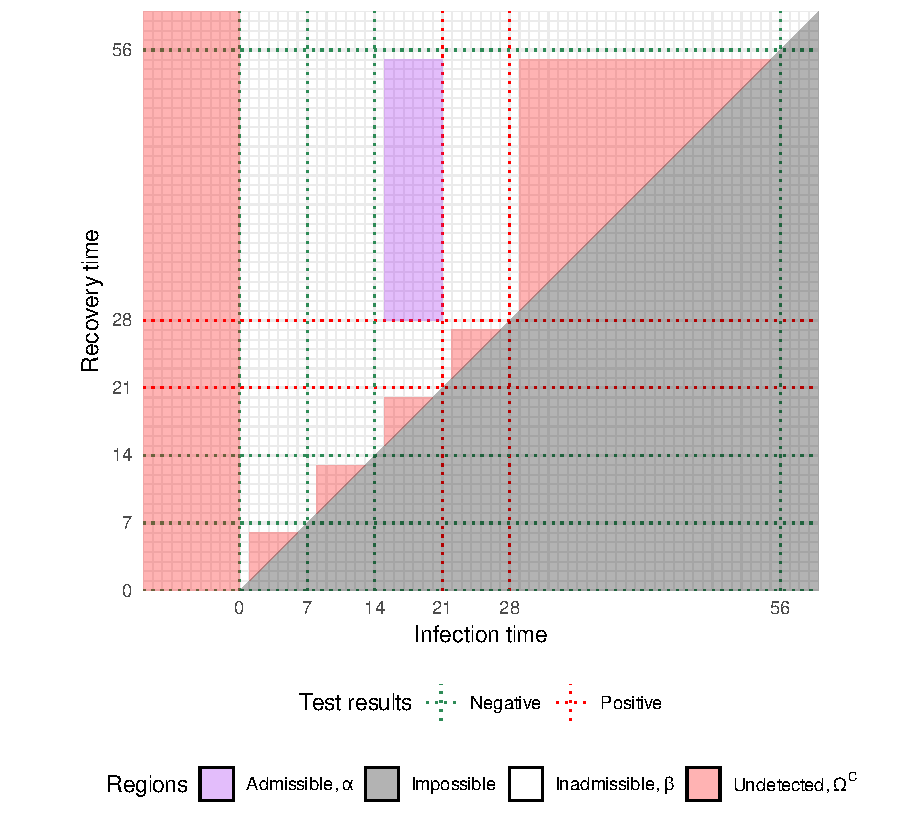
\includegraphics[width=\textwidth]{cis-perfect-testing/regions_diag}
\caption[Admissible, inadmissible, and undetected regions]{%
  The regions for individual $i$.
  $i$'s first test was at time 0 and negative, with subsequent negative tests at times 7, 14, and 56, and positive tests at times 21 and 28.
  Inadmissible regions are unshaded.
  The black (impossible) region covers the cases in which recovery occurs prior to infection.
  \label{perf-test:fig:partitionSpace}
}
\end{figure}

These three classes span all possible episodes and are mutually exclusive.
Hence, $\ntot = \ndet + \nnodet + n_{i\bar{a}} = \sum_{i=1}^{\Ncis} n_{ia} + \sum_{i=1}^{\Ncis} n_{iu} + 0$.
Furthermore, for all $i$, $p_{ia} + p_{iu} + p_{i\bar{a}} = 1$.

% Any episode $j$ independently belongs to one of these classes.
The probabilities ($p_{iu}$, $p_{ia}$, and $p_{i\bar{a}}$), are conditional on the episode occurring in individual $i$.
I assume the individual in which each episode occurs is iid uniform across the cohort.
Therefore, the unconditional probabilities of an infection belonging to a class need to be multiplied by $1/\Ncis$.
For example, the probability of an episode being in class $\alpha_i$ is $p_{ia} / \Ncis$.

Each episode occurs in one of the classes independently and with the same probability.
Therefore, conditional on $\ntot$, the number of episodes in each class is multinomial.
Specifically:
\begin{align}
  \begin{bmatrix}
    n_{1a} \\ n_{1u} \\ n_{1\bar{a}} \\ \vdots \\ n_{\Ncis,a} \\ n_{\Ncis,u} \\ n_{\Ncis,\bar{a}}
  \end{bmatrix}
  \mid \ntot
  =
  \MN\left(
    \ntot,
    \frac{1}{\Ncis}
    \begin{bmatrix}
      p_{1a} \\ p_{1u} \\ p_{1\bar{a}} \\ \vdots \\ p_{\Ncis,a} \\ p_{\Ncis,u} \\ p_{\Ncis,\bar{a}}
    \end{bmatrix}
  \right)
  \label{perf-test:eq:multinomial}
\end{align}

In forming the region $\alpha_i$, I use the test outcomes.
This is not strictly correct because the cell probabilities in the likelihood should not depend on the data.
However, an alternative where each combination of infection and recovery times is considered its own cell is possible.
The new cells would align with the inadmissible region.
Since each of these cells have an observed count of 0, they can be combined to give the same likelihood.
That is, the approach is mathematically equivalent but greatly complicates the formulae and notation.
Therefore, I present this version as it is clearer.

The undetected classes cannot be distinguished.
Therefore, these classes can be combined into a single class.
The combined class has a count $\nnodet = \sum_{i=1}^{\Ncis} n_{iu}$ and probability $\pnodet = \frac{1}{\Ncis} \sum_{i=1}^{\Ncis} p_{iu}$.

\subsection{Posterior density} \label{perf-test:sec:posterior-density}

Let $\na = (n_{1a}, \dots, n_{\Ncis a})^T$ be the vector of counts of episodes in the admissible classes.
This represents all the observations used in \cref{perf-test:eq:multinomial}.
Therefore, the posterior density we are interested in is $p(\vec{\theta} \mid \na)$.
It can be written as follows.
\begin{align}
p(\vec{\theta} \mid \na)
&\propto p(\vec{\theta}) p(\na \mid \vec{\theta}) \\
&= p(\vec{\theta}) \sum_{\ntot=\ndet}^\infty p(\ntot \mid \vec{\theta}) p(\na \mid \ntot, \vec{\theta})
\label{perf-test:eq:posterior1}
\end{align}
where the last line augments the likelihood with the total number of episodes, $\ntot$.

First, I derive the form of $p(\na \mid \ntot, \vec{\theta})$.
From \cref{perf-test:sec:episode-types}, the counts $\na$ and $\nnodet$'s joint distribution, conditional on $\ntot$, is multinomial.
All $n_{i\bar{a}} = 0$, therefore these classes can be ignored; counts of zero do not contribute to the multinomial probability mass function (they multiply by 1).
The support of the distribution requires $\nnodet = \ntot - \sum_{i=1}^{\Ncis} n_{ia} = \ntot - \ndet$ and $\ntot \geq \ndet$.
Hence:
\begin{align}
p(\na \mid \ntot, \vec{\theta})
&= p(\nnodet  = \ntot - \na, \na\mid \ntot, \vec{\theta}) \\
&= \frac{\ntot!}{(\ntot - \ndet)! \prod_{i=1}^{\Ncis} n_{ia}!}  \pnodet^{\ntot - \ndet}\prod_{i=1}^{\Ncis} \left(\frac{1}{\Ncis}p_{ia}\right)^{n_{ia}} \\
&\propto \frac{\ntot!}{(\ntot - \ndet)!} \pnodet^{\ntot - \ndet} \prod_{i \in \set{D}} p_{ia} \label{perf-test:eq:augmented-likelihood}
\end{align}
the final line follows because $n_{ia} = 1$ for $i \in \set{D}$ and $n_{ia} = 0$ otherwise.

Substituting \cref{perf-test:eq:augmented-likelihood} into \cref{perf-test:eq:posterior1}:
\begin{align}
&\propto p(\vec{\theta}) \sum_{\ntot=\ndet}^\infty \left( p(\ntot \mid \vec{\theta}) \frac{\ntot!}{(\ntot - \ndet)!} \pnodet^{\ntot - \ndet} \prod_{i \in \set{D}} p_{ia} \right) \\
&= p(\vec{\theta}) \left( \prod_{i \in \set{D}} p_{ia} \right) \left( \sum_{\ntot=\ndet}^\infty p(\ntot \mid \vec{\theta}) \frac{\ntot!}{(\ntot - \ndet)!} \pnodet^{\ntot - \ndet} \right) \label{perf-test:eq:posterior2}.
\end{align}
For convenience, define the summation term as:
\begin{align}
  \eta =  \sum_{\ntot=\ndet}^\infty p(\ntot \mid \vec{\theta}) \frac{\ntot!}{(\ntot - \ndet)!} \pnodet^{\ntot - \ndet}.
  \label{perf-test:eq:eta}
\end{align}
The rest of this section derives expressions for each of $p_{ia}$, $p_{u}$ and $\eta$.

\subsection{Expression for $\eta$}

I derive an analytical solution to $\eta$ under the prior $\ntot \dist \NBc(\mu, r)$.
I assume that $\vec{\theta}$, which are only the parameters of the survival distribution, has a prior independent of $\ntot$, the number of infections that occurred in the cohort.
Therefore, $p(\ntot \mid \vec{\theta}) = p(\ntot)$.

Putting a negative binomial prior on $\ntot$ is equivalent to the following gamma-Poisson composite; its use simplifies the derivation.
\begin{align}
\ntot \mid \lambda &\dist \Poi(\lambda) \\
\lambda &\dist \GamDist(a, b)
\end{align}
where $b = r / \mu$ and $a = r$.
Hence:
\begin{align}
\eta
&= \int \sum_{\ntot=\ndet}^\infty \frac{\ntot!}{(\ntot-\ndet)!} \pnodet^{\ntot-\ndet} p(\ntot \mid \lambda) p(\lambda) d\lambda &\text{$\lambda$ explicit}\\
&= \int \sum_{\ntot=\ndet}^\infty \frac{\ntot!}{(\ntot-\ndet)!} \pnodet^{\ntot-\ndet} \frac{\lambda^{\ntot} e^{-\lambda}}{\ntot!} p(\lambda) d\lambda &\ntot \dist \Poi\\
%&= \int \sum_{\ntot=\ndet}^\infty \frac{1}{(\ntot-\ndet)!} \pnodet^{\ntot-\ndet} \lambda^{\ntot-\ndet} \lambda^{\ndet} e^{-\lambda} p(\lambda) d\lambda \\
&= \int \lambda^{\ndet} e^{-\lambda} p(\lambda) \sum_{\nnodet=0}^\infty \frac{(\pnodet \lambda)^{\nnodet}}{\nnodet!} d\lambda &\nnodet = \ntot-\ndet\\
&= \int \lambda^{\ndet} e^{-\lambda} p(\lambda) e^{\lambda \pnodet} d\lambda &\text{Maclaurin series of $e$} \\
&= \int \lambda^{\ndet} e^{-\lambda(1 - \pnodet)} \frac{b^a}{\Gamma(a)} \lambda^{a-1} e^{-b\lambda} \lambda d\lambda &\text{Gamma pdf}\\
&= \int \frac{b^a}{\Gamma(a)} \lambda^{a+\ndet-1} e^{-(b+1-\pnodet)\lambda} \lambda d\lambda \\
&= \frac{b^a}{\Gamma(a)} \frac{\Gamma(a+\ndet)}{(b+1-\pnodet)^{a+\ndet}} &\text{Gamma pdf}\\
&\propto (b+1-\pnodet)^{-(a+\ndet)} \\
&= (r/\mu + 1 - \pnodet)^{-(r+\ndet)} &\text{sub in $\mu$ and $r$}\\
&\propto(r + \mu (1- \pnodet))^{-(r+\ndet)}.
\end{align}

Substituting this into \cref{perf-test:eq:posterior2} gives:
\begin{align}
p(\vec{\theta} \mid \na)
&\propto p(\vec{\theta}) \left( \prod_{i \in \set{D}} p_{ia} \right) (r + \mu (1- \pnodet))^{-(r+\ndet)} \label{perf-test:eq:full-posterior}.
\end{align}

% $\ntot$ is generally a nuisance parameter, however, its posterior distribution can be useful for diagnostic purposes (as in X\todo{ref where I use this in the next chapter}).
% Its posterior can be reconstructed using a posterior sample of $\vec{\theta}$.
% For each posterior sample of $\vec{\theta}$, sample from the full conditional of $\ntot$ to give the joint posterior of $\ntot$ and $\vec{\theta}$.
% The full conditional of $\ntot$ is given by:
% \begin{align}
% p(n_\text{tot} \mid \ncis, \vec{\theta})
% &\propto p(\ntot \mid \vec{\theta}) p(\ncis \mid \vec{\theta}, \ntot) \\
% &\propto p(\ntot \mid \vec{\theta}) \frac{\ntot!}{(\ntot - \ndet)!} \pnodet^{\ntot - \ndet} &\text{by \cref{perf-test:eq:augmented-likelihood}} \\
% &\propto \frac{\Gamma(r + \ntot)}{\ntot!} \left( \frac{\mu}{r + \mu} \right)^{\ntot} \frac{\ntot!}{(\ntot-\ndet)!} \pnodet^{\ntot} \\
% &= \frac{\Gamma(r + \ntot)}{(\ntot-\ndet)!} \left( \frac{\mu \pnodet}{r + \mu} \right)^{\ntot}  \\
% &= \frac{\Gamma((r + \ndet) + (\ntot- \ndet))}{(\ntot-\ndet)!} \left( \frac{\mu \pnodet}{r + \mu} \right)^{\ntot-\ndet}.
% \end{align}
% Comparing this expression to the pmf of a negative binomial, we find that $\nnodet = \ntot - \ndet$ is distributed negative binomial with size parameter $r+\ndet$ and probability parameter $(r + \mu(1 - \pnodet))/(r + \mu)$.
%The mean of this distribution is $(r+\ndet)\mu \pnodet/(r+\mu(1-\pnodet))$.

\subsection{Admissible probabilities}

Next, I derive $p_{ia}$.
From \cref{perf-test:eq:full-posterior}, this is only needed for $i \in \set{D}$, that is for individuals with detected episodes.
For such an individual, let $j$ denote their detected episode.

By definition (see \cpageref{perf-test:def:admissible}), we have, for any $i \in \set{D}$:
\begin{align}
p_{ia} =& \prob((B_j, E_j) \in \alpha_i \mid \vec{\theta}, i(j) = i) \\
\alpha_i =& \{ (b, e) : l_{j}^{(b)} \leq b \leq r_{j}^{(b)} \wedge l_{j}^{(e)} \leq e \leq r_{j}^{(e)}\}.
\intertext{Omitting the conditioning on $\vec{\theta}$ and $i(j) = i$, this gives:}
p_{ia}
=& \prob \left( l_{j}^{(b)} \leq B_{j} \leq r_{j}^{(b)}, l_{j}^{(e)} \leq E_{j} \leq r_{j}^{(e)} \right) \\
=& \prob \left( l_{j}^{(e)} \leq E_{j} \leq r_{j}^{(e)} \mid l_{j}^{(b)} \leq B_{j} \leq r_{j}^{(b)} \right) \\
   &\times\prob \left( l_{j}^{(b)} \leq B_{j} \leq r_{j}^{(b)} \right) \\
=& \sum_{b = l_{j}^{(l)}}^{r_{j}^{(b)}} \prob \left( l_{j}^{(e)} \leq E_{j} \leq r_{j}^{(e)} \mid B_{j} = b \right) \prob \left(B_{j} = b \right) \\
=& \sum_{b = l_{j}^{(b)}}^{r_{j}^{(b)}} \prob \left( l_{j}^{(e)} - b + 1 \leq D_{j} \leq r_{j}^{(e)} - b + 1 \right) \prob \left(B_{j} = b \right) &\text{by def of $D_{j}$} \\
=& \sum_{b = l_{j}^{(b)}}^{r_{j}^{(b)}} \left( S_{\vec{\theta}}(l_{j}^{(e)} - b + 1) - S_{\vec{\theta}}(r_{j}^{(e)} - b + 2) \right) \prob \left(B_{j} = b \right) &\text{by def of $S_{\vec{\theta}}$} \\
\propto& \sum_{b = l_{j}^{(b)}}^{r_{j}^{(b)}} \left( S_{\vec{\theta}}(l_{j}^{(e)} - b + 1) - S_{\vec{\theta}}(r_{j}^{(e)} - b + 2) \right)
\end{align}
under the assumption of uniform probability of infection time.
This is the standard form of the likelihood for doubly interval censored data without truncation~\autocite[e.g.][]{sunEmpirical}.

\subsection{Undetected probability} \label{perf-test:sec:prob-undetected}

The final component of \cref{perf-test:eq:full-posterior} required is $1 - p_u$.
From \cref{perf-test:sec:episode-types}:
\begin{align}
  1 - p_u
  &= 1 - \frac{1}{\Ncis} \sum_{i=1}^{\Ncis} p_{iu} \\
  &= \frac{1}{\Ncis} \sum_{i=1}^{\Ncis} (1 - p_{iu}).
  \label{perf-test:eq:pu}
\end{align}

Therefore, the crucial component is $1 - p_{iu} = 1 - \prob((B_j, E_j) \in \Omega_i \mid \vec{\theta}, i(j) = i)$.
This is one minus the probability that an episode in individual $i$ was undetected, \ie the probability that episode such an episode is detected.

An episode $j$ in individual $i(j)$ is detected if and only if all the following conditions are met.
\begin{enumerate}
    \item $\exists t \in \sched_{i(j)}$ such that $b_j \leq t \leq e_j$; this condition is equivalent to having at least one positive test for the episode.
    \item $\exists t \in \sched_{i(j)}$ such that $t < b_j$.
      For individuals enrolled during the period considered ($\min \sched_{i(j)} > 0$), this ensures that the beginning of the episode is lower bounded; thereby adjusting for those who enrolled during the period being less likely to have a detected infection.
      For individuals enrolled prior to the period considered ($\min \sched_{i(j)} \leq 0$), this means that the episode was not detected prior to time 1.
    \item $\exists t \in \sched_{i(j)}$ such that $t \geq b_j$.
      This means that the test is detected before $T$.
    \item $\exists t \in \sched_{i(j)}$ such that $t > e_j$, upper bounding the end of the episode.
      For episodes detected in the period I consider, this happens a negligible number of times, only in individuals lost to follow-up; therefore, I neglect this possibility.
      For a new context, including recent infections, this condition could be relaxed by considering episodes that do not meet this criteria as right censored.
\end{enumerate}

% An episode is undetected if and only if no tests are performed during the episode or if there was no negative test prior to the episode.
% Equivalently, that the first test at or after $b$ is after $e$, or that there is no negative test prior to $b$.
To formalise this, first define $\tau_{\sched_i}(t)$ as the time until the next test at or after time $t$ in the schedule $\sched_i$:
\begin{align}
\tau_{\sched_i}(t) &= \min \{ t' \in \sched_i : t' \geq t \} - t
\end{align}
defining $\min \emptyset = \infty$; \ie $\tau_{\sched_i}(t) = \infty$ if there is no $t' \in \sched_i$ such that $t' \geq t$.
The condition that $\exists t \in \sched_{i(j)}$ such that $b_j \leq t \leq e_j$ can now be expressed as $e_j \geq b_j + \tau_{\sched_{i(j)}}(b_j)$.
Equivalently, $d_j \geq \tau_{\sched_{i(j)}}(b_j) + 1$.


% Then $\Omega_i$ can be written as:
% \begin{align}
% \Omega_i = \{ (b, e) \ssep \tau_{\sched_i}(b) + b > e \vee b \leq \min(\sched_i) \}.
% \end{align}
Therefore, omitting the conditioning on $\vec{\theta}$ and $i(j) = i$:
\begin{align}
1 - p_{iu}
&= 1 - \prob((B_{j}, E_{j}) \in \Omega_i) \\
&= \prob(D_j \geq \tau_{\sched_{i}}(B_j)+ 1, B_j > \min \sched_{j}) \\
&= \sum_{b = \min \sched_{i} + 1}^T \prob(D_j \geq \tau_{\sched_{i}}(b) + 1 \mid B_j = b) \prob(B_j = b)\\
&= \frac{1}{T} \sum_{b = \min \sched_{i} + 1}^T S_{\vec{\theta}}(\tau_{\sched_{i}}(b) + 1)
\end{align}
defining $S_{\vec{\theta}}(\infty) = 0$.

Substituting into \cref{perf-test:eq:pu}:
\begin{align}
1 - p_u
& \propto \sum_{i=1}^{\Ncis} \sum_{b = \min \sched_{i} + 1}^T S_{\vec{\theta}}(\tau_{\sched_{i}}(b) + 1)
\end{align}

\section{Parameterisation and priors for the survival function} \label{perf-test:sec:parameters-priors}

In this section I specify the form of $S_{\vec{\theta}}(t)$.
I parameterize $S$ in terms of the hazard $S_{\vec{\theta}}(t) = \prod_{i=1}^{t-1} (1 - \lambda(i))$ (see \cref{E-inc-prev:sec:definitions}).
Therefore, $\vec{\theta} = [\lambda_1, \dots, \lambda_{\dmax-1}]^T$.

Priors cannot be vague on both the hazard and the survival, the implications of which I consider in what follows.
Informative priors are also attractive to allow the incorporation of the estimates from \cref{E-ATACCC}.

\subsection{Independent priors} \label{perf-test:sec:independent-priors}
Take the standard assumption of independent priors on each parameter.
Each hazard, $\lambda_t$, is a (conditional) probability, and hence a Beta distribution is a natural choice.

Uninformative Beta priors on the hazard are problematic in this context.
An uninformative prior would be of the form $\lambda_t \dist \BetaDist(\alpha, \alpha)$.
Commonly, $\alpha$ is chosen to be $0.5$ (Jeffreys' Prior) or $1$ (a uniform prior).
Even though these priors are uninformative on the hazard, they become highly informative on the survival. 
Specifically, they tend to favour shorter survival times (see \cref{perf-test:fig:flat-prior}).
An intuitive explanation of this follows from the fact that priors of this form have an expected value of 0.5.
The expected survival time, $\E \left( \prod_{i=1}^{t-1} (1-\lambda_t) \right)$, is therefore equal to $0.5^{t-1}$, a quantity that declines rapidly.
This prior expresses extreme scepticism in estimates from previous studies, such as \cref{E-ATACCC} and the meta-analysis of \textcite{cevikShedding}.
\begin{figure}
  \centering 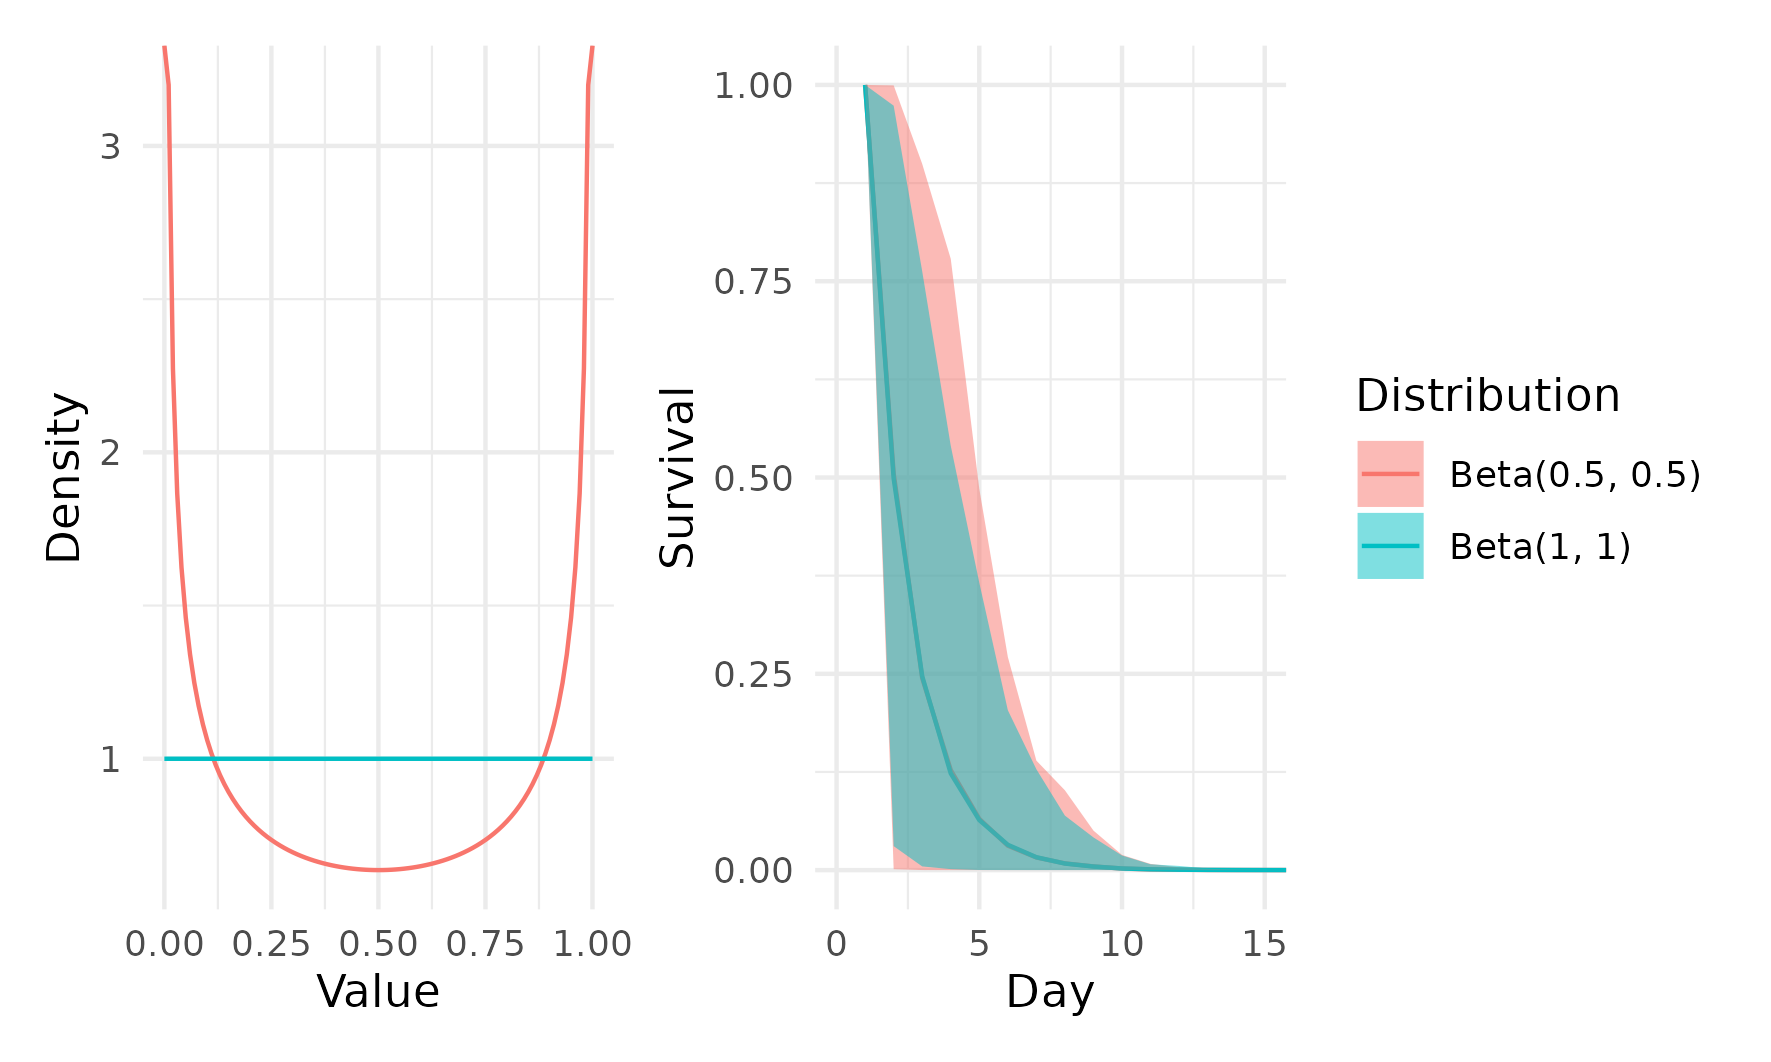
\includegraphics{cis-perfect-testing/flat-prior}
  \caption[Uninformative priors for the hazard]{
    (A) Density of Beta(1, 1) flat prior and Beta(0.5, 0.5) uninformative priors.
    (B) Prior predictive survival time (mean and 95\% CrI).
    The implied prior on the survival time is very short when using either prior on the hazard at each time.
  }
 \label{perf-test:fig:flat-prior}
\end{figure}

Instead, I propose a weakly informative (or vague) prior Beta(0.1, 1.9), which has mean 0.05 and minimal information.
The amount of information in a Beta distribution is related to the sum of its parameters.
Here, the sum equals 2, the same as the flat prior case.
The central 95\% probability mass of Beta(0.1, 1.9) is 0.00--0.47.
The central estimate, of 0.05, is in line with previous estimates that the median duration in the range 15--20 days~\autocite{cevikShedding}.
This prior gives a very vague prior predictive distribution on the survival time (see \cref{perf-test:fig:vague-prior}).
\begin{figure}
  \centering 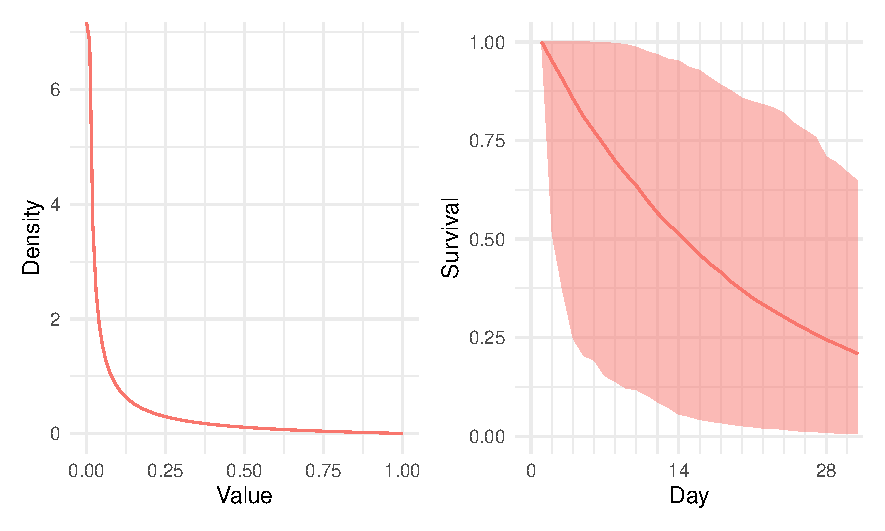
\includegraphics{cis-perfect-testing/vague-prior}
  \caption[Vague prior for the hazard]{
    (A) Density of Beta(0.1, 1.9) vague prior.
    (B) Prior predictive survival time (mean and 95\% CrI).
    Note the different x-axis to \cref{perf-test:fig:flat-prior}.
  }
  \label{perf-test:fig:vague-prior}
\end{figure}


\subsection{Smoothing priors}

Smoothing priors~\autocite{gerschSmoothness} encode the biological consideration that the hazard should not vary significantly from day-to-day.
They serve the same purpose as a penalized likelihood, which is used frequently in the non-parametric maximum-likelihood setting~\autocite[e.g.][]{bacchettiNonparametric}.
Many possible forms of smoothing priors exist, including splines, Gaussian Processes, and random walks.
I use a second-order random walk (RW2) because it is simple and produces sensible prior predictive distributions.

RW2 prior encodes that the hazard should be linearly changing with some random changes at each time step.
Specifically, the difference on the logit scale between $\lambda_t$ to $\lambda_{t+1}$ is the difference between $\lambda_{t-1}$ and $\lambda_t$ plus some normally distributed noise.
Formally:
\begin{align}
  \logit\lambda_{t+1}
  &= \logit\lambda_t + (\logit\lambda_t - \logit\lambda_{t-1}) + \sigma \epsilon_t &\text{for $t \geq 2$} \\
  &= 2\logit\lambda_t - \logit\lambda_{t-1} + \sigma \epsilon_t \\
  \epsilon_t &\dist \N(0, 1) &\text{for $t \geq 2$}  \\
  \logit\lambda_2 &= \logit\lambda_1 + \epsilon_1 \\\
  \epsilon_1 &\dist \N(\mu_{\epsilon_1}, \sigma_{\epsilon_1}^2) \\
  \logit \lambda_1 &\dist \N(\mu_{\lambda_1}, \sigma_{\lambda_1}^2) \\
  \sigma &\dist \Exponential(1/\mu_\sigma).
\end{align}
The hyperparameters $\mu_{\lambda_1}$ and $\sigma_{\lambda_1}$ specify the prior on the hazard at time 1; $\mu_{\epsilon_1}$ and $\sigma_{\epsilon_1}$ specify the prior on the initial gradient, $\lambda_2 - \lambda_1$; and $\mu_\sigma$ specifies the smoothness of the random walk.
I use $\mu_{\lambda_1} = -17.5$, $\sigma_{\lambda_1} = 6$, $\mu_\epsilon = 1.09$, $\sigma_\epsilon = 0.03$, and $\mu_\epsilon = 0.1$ based on the analysis in \cref{E-ATACCC} (see \cref{perf-test:fig:rw2-prior}).
\begin{figure}
  \centering 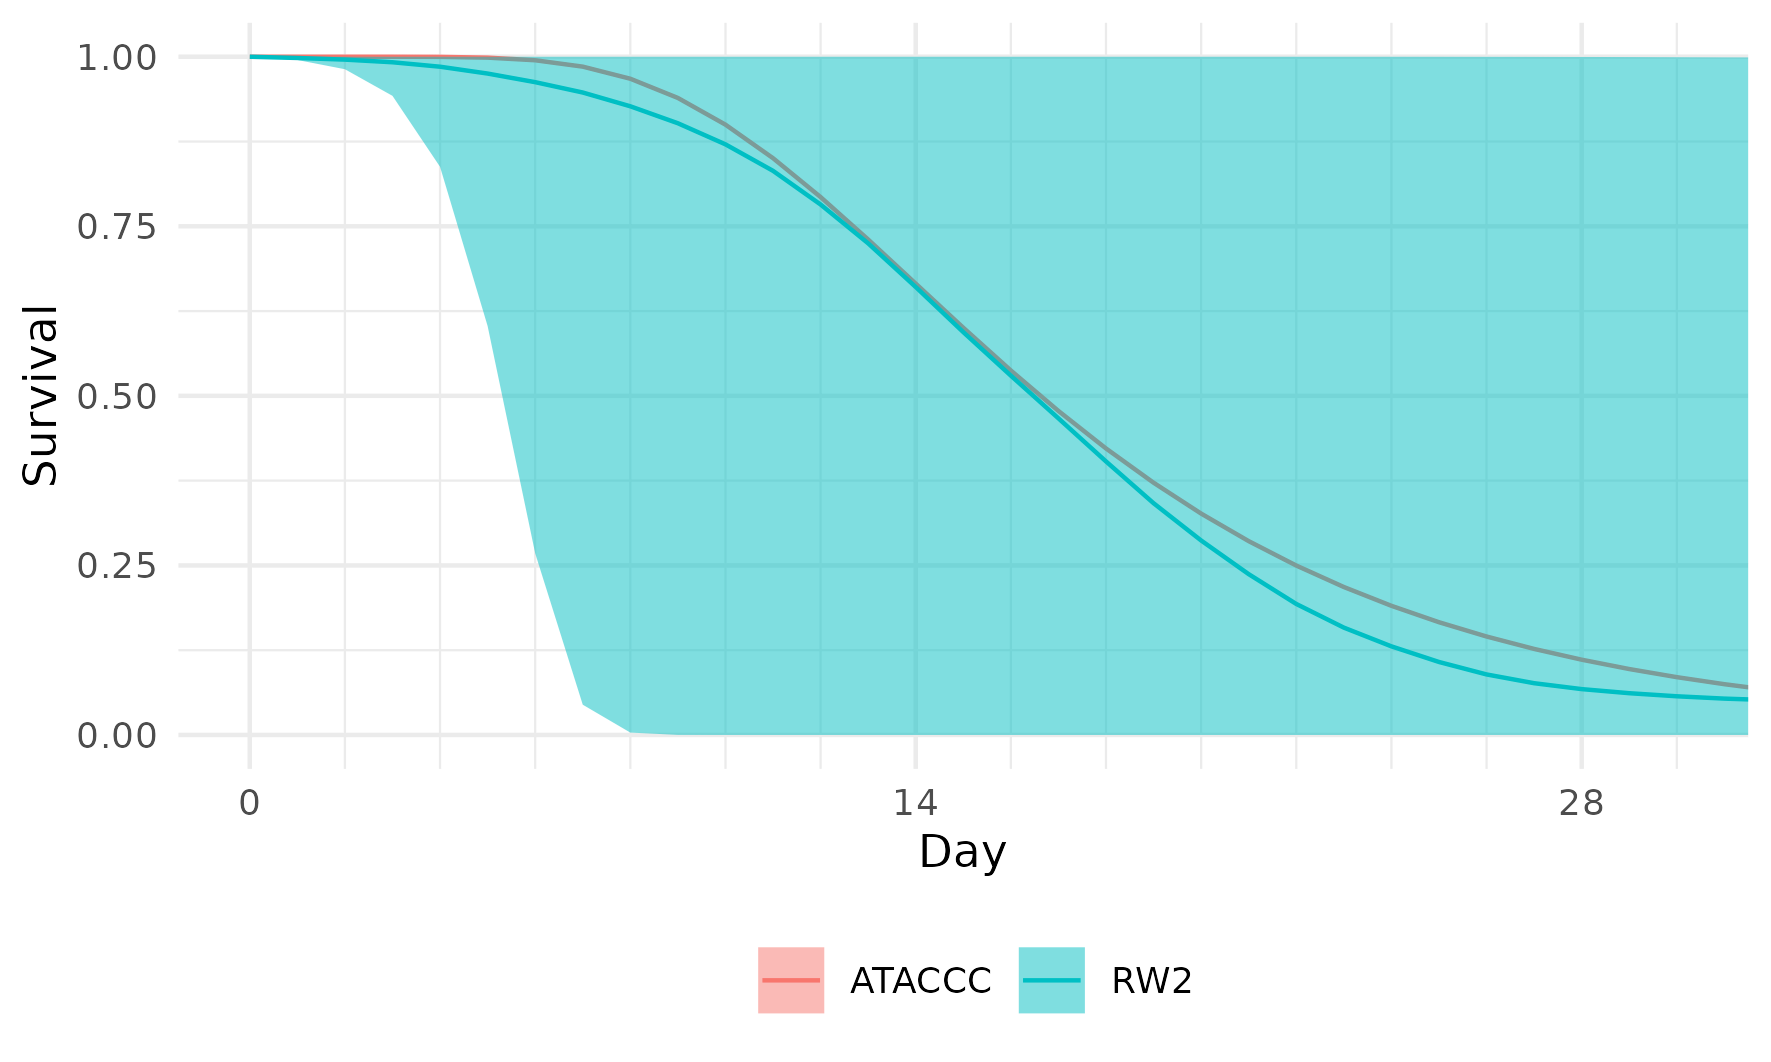
\includegraphics{cis-perfect-testing/rw2-prior}
  \caption[RW2 prior for the hazard]{The prior predictive survival time (mean and 95\% central interval) for the RW2 prior specified in the main text. The posterior mean estimate using ATACCC data in \cref{E-ATACCC} is shown for comparison. \label{perf-test:fig:rw2-prior}}
\end{figure}

\subsection{Model combination priors} \label{perf-test:sec:informative-priors}

The information from \cref{E-ATACCC} can be incorporated through the prior.
This is desirable because the ATACCC study frequently sampled individuals for around the first 20 days of their infection.
Therefore, the first 20 days of \cref{E-ATACCC}'s estimate of the survival distribution is reliable.
The CIS data can then inform the posterior after this point.

When constructing the prior, two aspects need consideration.
Firstly, the model structure from \cref{E-ATACCC} leads to positive correlation in the posterior estimates of the hazard, which should be propagated into this analysis.
That is, the prior used in this analysis cannot be independent across the hazards.
Secondly, the uncertainty in the estimates from \cref{E-ATACCC} is underestimated because it extrapolates beyond the data using strong model assumptions (see \cref{E-ATACCC:sec:discussion}).
%Furthermore, there are differences in the study design and laboratories used between the two studies (see \cref{E-intro:sec:studies}) which may mean that results do not generalise between the studies.
I form the prior to include this prior information into the CIS analysis two steps.

I first approximate the \cref{E-ATACCC} posterior estimate of the hazard as $\logit{\vec{h}} \dist \MNorm(\vec{\mu}_A, \matr{\Sigma}_A)$ where $\vec{h}$ is the posterior distribution of the hazards, and $\vec{\mu}_A$ and $\matr{\Sigma}_A$ are the mean and covariance matrix computed from the samples of $\logit{\vec{h}}$ derived using the method of \cref{ATACCC:sec:duration}.
Using a multivariate normal, as opposed to multiple univariate distribution for each $h_t$, preserves the correlation between the hazards.
The logit transformation maps from the $[0, 1]$ interval to the full real line.
The approximation is very good (see \cref{perf-test:fig:approximate-ATACCC-hazard} and \cref{perf-test:fig:approximate-ATACCC-survival}).
\begin{figure}
  \thisfloatpagestyle{empty}
  % \vspace{-1cm}
  \makebox[\textwidth][c]{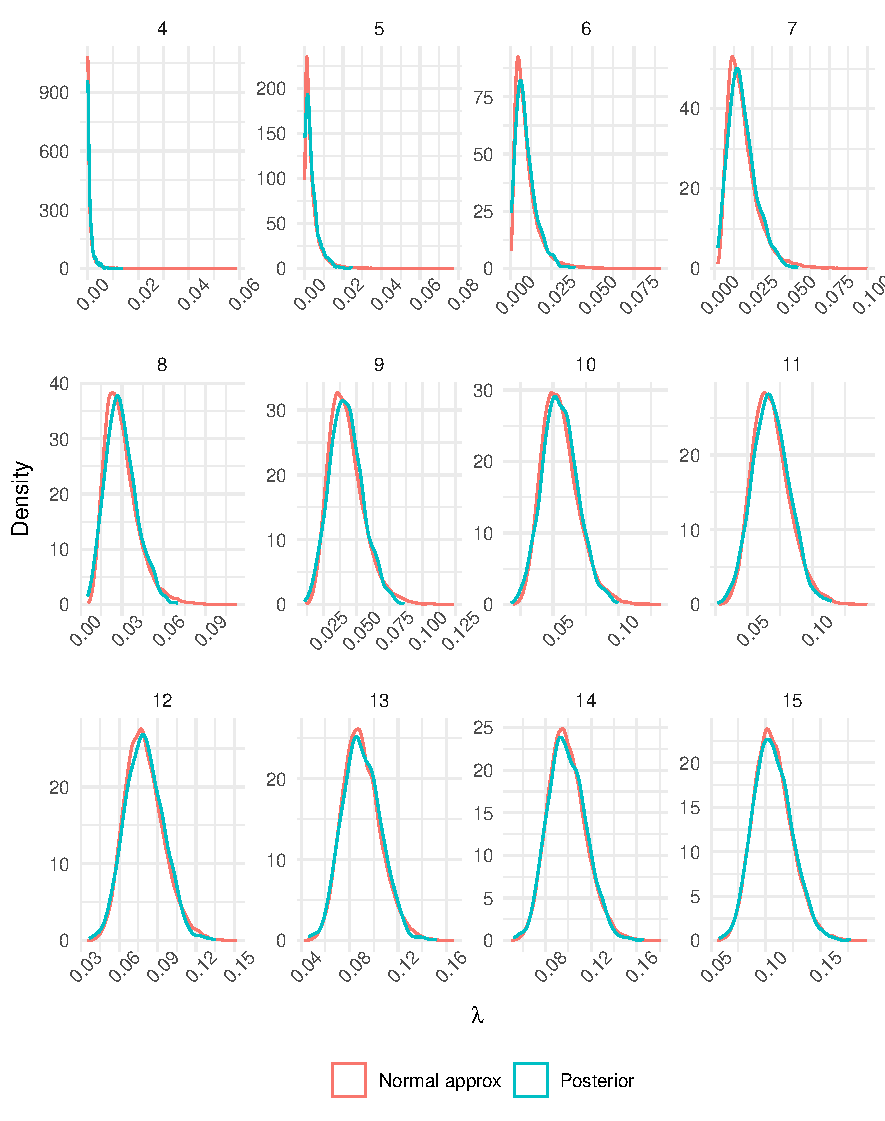
\includegraphics[width=.9\paperwidth]{cis-perfect-testing/ataccc-approximation-hazard}}
  \caption[Approximating the ATACCC posterior hazard as a logit-normal]{Comparison of the posterior estimate of the hazard from \cref{E-ATACCC} and its approximation with a logit-normal distribution (kernel density estimate smoothed) for hazards between day 4 and 15. The density for smaller hazards is concentrated very close to 0. \label{perf-test:fig:approximate-ATACCC-hazard}}
\end{figure}
\begin{figure}
  \centering 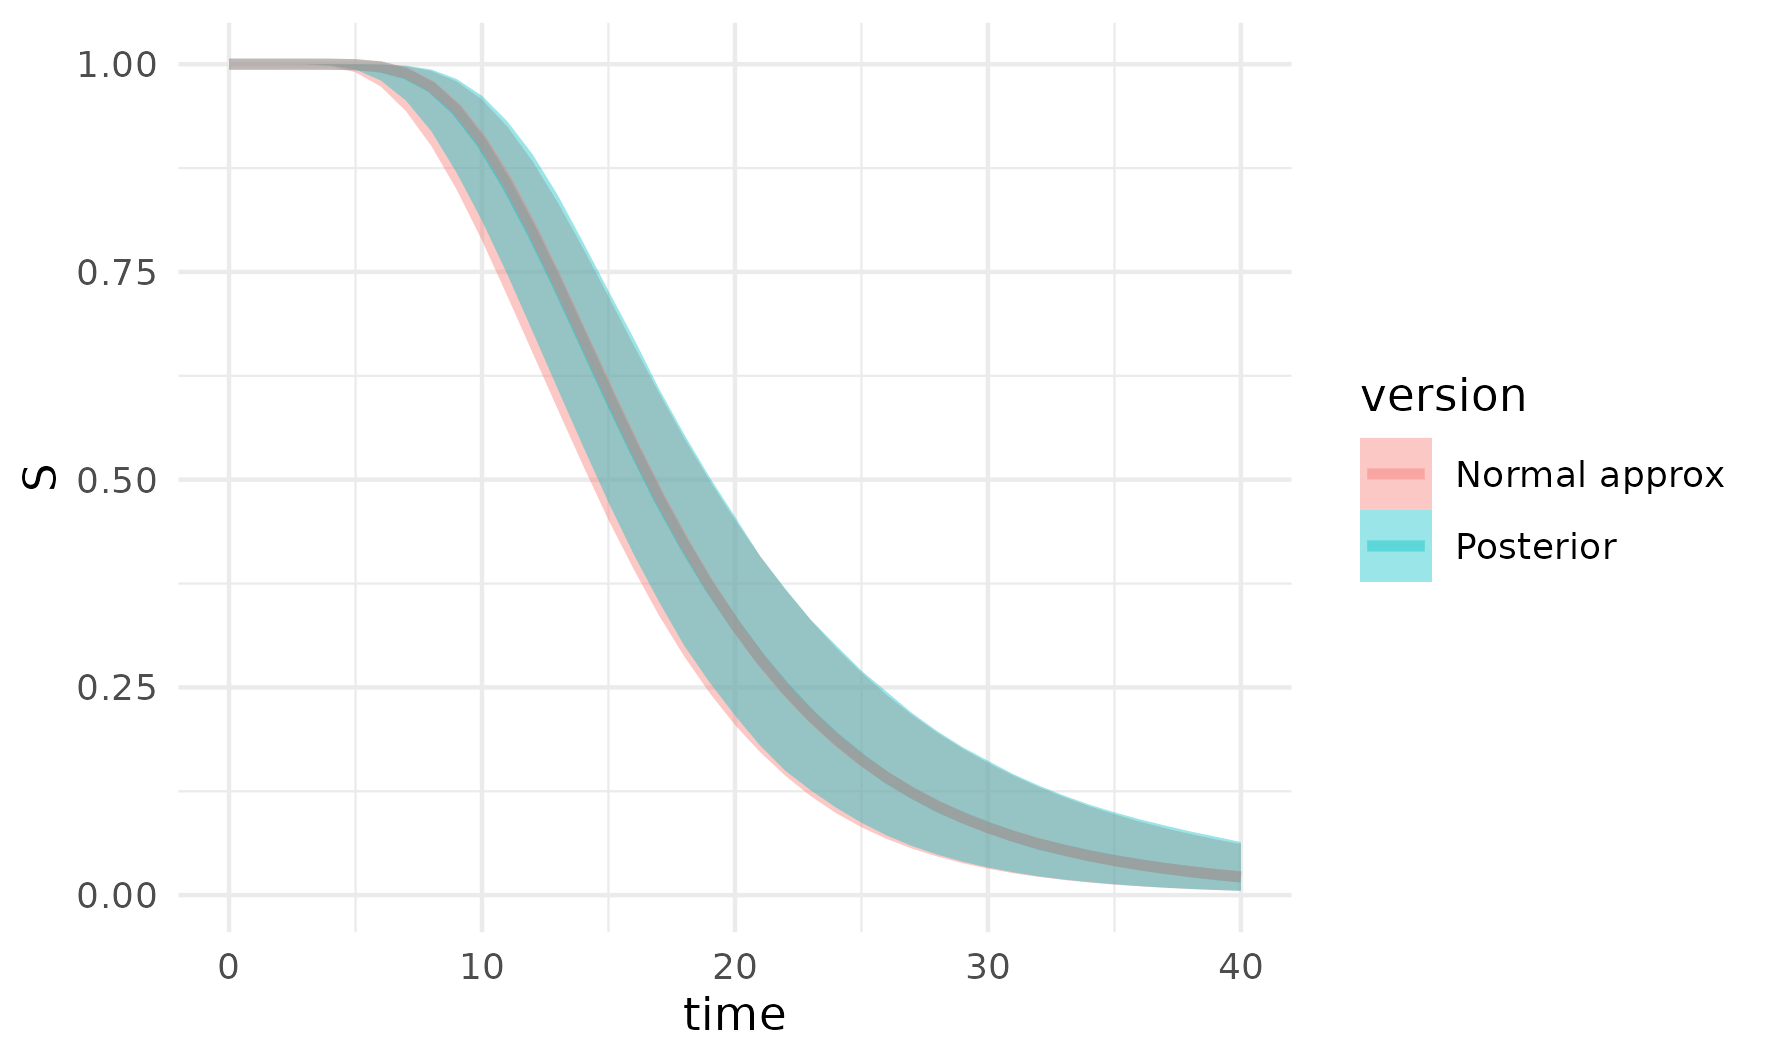
\includegraphics{cis-perfect-testing/ataccc-approximation-survival}
  \caption[Approximating the ATACCC posterior survival as a logit-normal]{Comparison of the posterior estimate of the survival from \cref{E-ATACCC} and its approximation with a logit-normal distribution (median and central 95\% interval). The survival is a function of all the hazards up until that point, therefore the correlation between the hazards must be well-approximated to have these agree. \label{perf-test:fig:approximate-ATACCC-survival}}
\end{figure}

Having approximated the estimate as a multivariate normal, I add additional uncertainty using a discrete Beta process.
The discrete Beta process prior generalises the form of prior used in \cref{perf-test:sec:independent-priors} by allowing the central estimate of the hazard to vary over time~\autocite{ibrahimBayesian,sunStatisticala}.
It is:
\begin{align}
  \logit \vec{h} &\dist \MNorm(\vec{\mu}_A, \matr{\Sigma}_A) \\
  \lambda_t &\dist \text{Beta}(\alpha_t, \beta_t) &t = 1, 2, \dots \\
  \alpha_t &= k_t h_t + \alpha_0 \\
  \beta_t &= k_t (1 - h_t) + \beta_0
\end{align}
where $k_t$, $\alpha_0$, and $\beta_0$ are hyperparameters; and $h_t$ is an estimate of the hazard at time $t$ from ATACCC.
An intuition for what this distribution represents derives from a conjugate model for $\lambda_t$ with a beta prior and a binomial likelihood.
If $\lambda_t$ is given the prior distribution $\text{Beta}(\alpha_0, \beta_0)$, and we then have $k_t$ observations with $k_t h_t$ successes, then the posterior distribution for $\lambda_t$ is $\text{Beta}(\alpha_t, \beta_t)$ (as defined above).

$k_t$ reflects the subjective belief that the estimates from \cref{E-ATACCC} are very reliable in the early infection period but unreliable by day 30.
The equation for $k_t$ is below and shown in \cref{perf-test:fig:kt}.
\begin{align}
k_t = \begin{cases}
  \expit(-0.4 * (t - 20)) &\text{for $t \leq 39$} \\
  0 &t > 39
\end{cases}
\end{align}
where $\expit(x) = 1 / (1 + \exp(-x))$.

\begin{figure}
  \centering 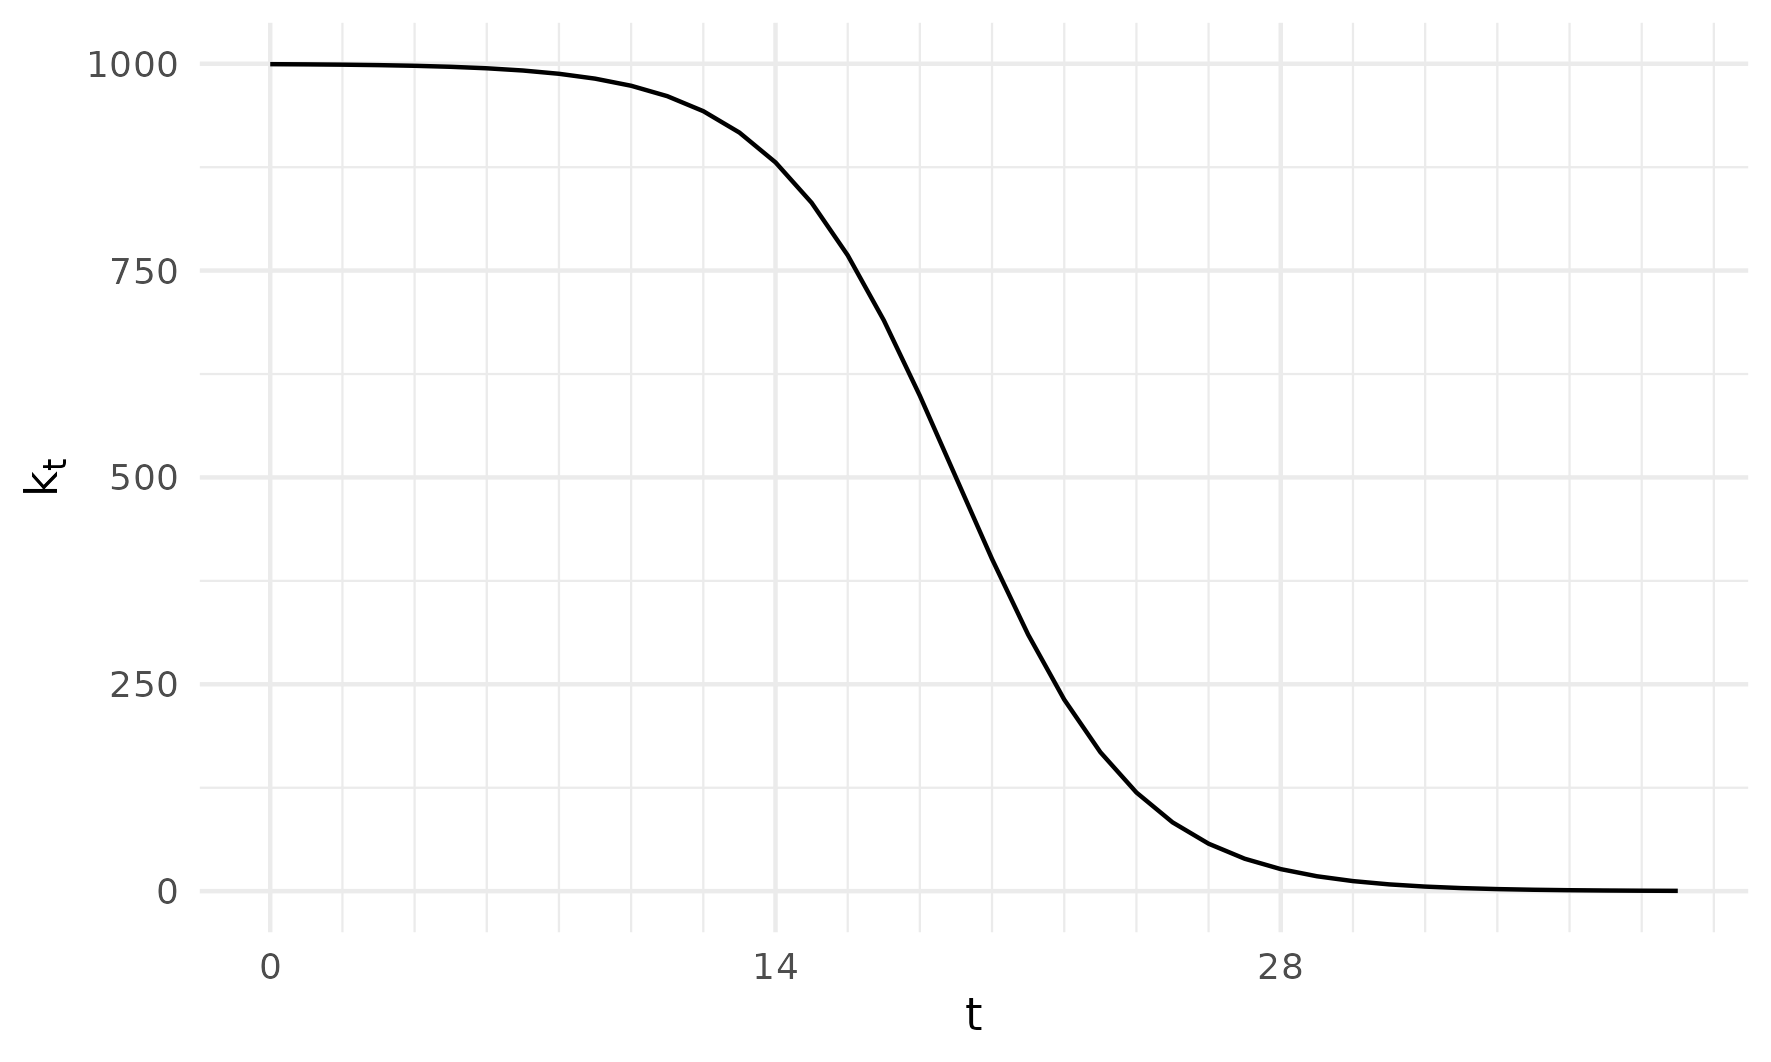
\includegraphics{cis-perfect-testing/kt-prior}
  \caption{Function used for $k_t$. \label{perf-test:fig:kt}}
\end{figure}

\section{Simulation study} \label{perf-test:sec:simulation-study}

\subsection{Setup}

I simulate a dataset of detected episodes with the same characteristics as that in the CIS by the following procedure.
\begin{enumerate}
    \item Extract the test schedules for each individual who had at least one test during the period of interest.
    \item Draw an episode start time, $b_{j}$ for each individual uniformly at random between 2nd July 2020 (100 days before the period where a detected episode would be included) and 6th December 2020 (the end of this period).
    \item Draw a duration of episode for each individual, $d_i$, based on the distribution described below. Then calculate the end of their infection episode, $e_{j} = b_{j} + d_i - 1$.
    \item Simulate the test results based on the test schedule, $b_{j}$, and $e_{j}$. Tests between $b_{j}$ and $e_{j}$ (inclusive) are positive, all other tests are negative.
    \item Discard episodes where there are no positive tests (\ie undetected episodes) and then apply the same inclusions/exclusions as in \cref{perf-test:sec:problem}.
    \item Of these remaining episodes, sample 4,800 to match the sample size of the true dataset. This is needed because in step 2 the entire cohort was infected, while in the real study only an (unknown) portion is infected.
    \item For this final set of episodes, calculate $(l_j^{(b)}, r_j^{b}, l_j^{(e)}, r_j^{(e)})$ by taking the day after the last negative prior to any positives, the first positive, the last positive, and the day before the negative following the last positive respectively.
\end{enumerate}

Step 3 requires a distribution of the duration of positivity.
I base this assumption on the estimate from \cref{E-ATACCC} with an inflated tail to be consistent with the CIS.
I modify the tail based on an unpublished analysis of CIS data~\citePersonalComms{A.\ Sarah Walker}.
Walker uses survival analysis to estimate the duration from CIS data.
This analysis assumes the initiating event is known, and equal to the episode’s detection time. 
It assumes the final event is interval censored between the time of the final positive test and the subsequent negative test, or right censored if a negative test has not yet been observed.
A flexible, spline-based form is used for the baseline survival function~\autocite{roystonSTPM,roystonFlexible} with covariates introduced via proportional odds.
By not accounting for either the undetected infections or the interval censoring of the initiating event, this analysis has competing biases which makes them hard to interpret~\autocite{cisMethodsONS}.

% \todo[inline]{The following seems important to justify why we can't just use these estimates but is also basically an aside}
% We know of two biases introduced from this analysis.
% \enquote{There is a bias in estimating the clearance distribution because the analysis used to estimate how long a person stays positive only starts from their first positive test.
% Since (most) people will have become positive on an earlier day, this will bias the clearance curves downwards (making the estimates too short).
% However, there is another bias due to the survey missing positive episodes entirely if they are short.
% This means that our dataset has fewer short positive episodes than in the population as a whole, and that the sample used to run the survival analysis is biased towards people with longer positive episodes.
% This will bias the clearance curves upwards (making the estimates too long).}~\autocite{cisMethodsONS}.

To form the duration distribution used in the simulation, we combine the two estimates.
The pdf over the first 30 days is proportional to the ATACCC estimate, with the rest proportional to this CIS-based estimates.
% The CIS-based estimates are shifted 3 days in order to make this smooth; this counteracts the above bias of missing the start of the infection (for times above 30 days, the other bias, missing short infections, is negligible). ERR... I'M NOT DOING THIS ANYMORE OH NO!!
Denote by $f_A(t)$ the distribution function estimated in \cref{E-ATACCC} and $f_C(t)$ that from the CIS-based estimates just derived.
Then define:
$$
f_S'(t) = \begin{cases}
	f_A(t) &t \leq 30 \\
	f_C(t) &t > 30
\end{cases}
$$
Then the distribution used in the simulation is the normalised version of this: $f_S(t) = f'_S(t)/\sum_i f_S'(i)$.
These curves and the combined curve are compared in \cref{perf-test:fig:duration-dist}.
Individual $i$'s duration of positivity, $D_i$, is then an independent draw from this distribution.
\begin{figure}
  \centering 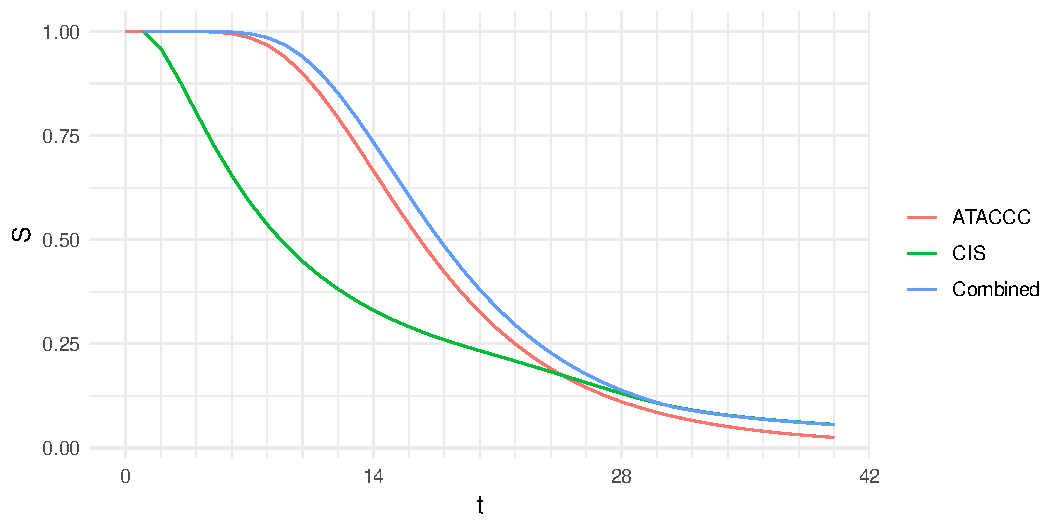
\includegraphics{cis-perfect-testing/input-duration-dists}
  \caption[Comparison of duration distributions]{Comparison of the duration distribution used for the simulation. ATACCC is the posterior mean from \cref{E-ATACCC}'s analysis, CIS is Sarah Walker's analysis, and Combined is the combination of these used for the simulation. \label{perf-test:fig:duration-dist}}
\end{figure}

\subsection{Implementation}

I implemented the simulation in R~4.2.0~\autocite{R-4-2-0} using tidyverse~2.0.0~\autocite{tidyverse} and targets~1.1.3~\autocite{targetsPackage}.

I implemented the inference in Stan via RStan~2.21.8~\autocite{rstan2-21-8} using default settings.
Convergence was assessed using Rhat and ESS as described in \cref{E-MCMC:sec:convergence}, and all runs checked for divergent transitions.

The prior on the total number of infections was centred on the true value with a dispersion parameter of 1.
This meant that the prior was very diffuse.


\subsection{Results} \label{perf-test:sec:results}

Repeating the simulation showed negligible variation in the results (not shown) due to the large sample size (4800 detected infections).
Therefore, I show and discuss results from only a single simulation.

All analyses converged.
Rhat were below 1.01, all parameters had an effective sample size of 1000, and there were no divergent transitions.

The true value of the survival function was generally well recovered (see \cref{perf-test:fig:survival-results}).
This was especially true for the first 30 days of the distribution.

The second-order random walk prior performed worst.
It showed oversmoothing, especially in the later parts of the distribution.
It smooths towards a linearly changing hazard; here, linearly decreasing (see \cref{perf-test:fig:hazard-results}).
This means that the survival function decreases slower than an exponential distribution in the tail.

The informative and vague independent priors performed similarly, with the informative prior having tighter credible intervals.
% The informative prior was centred on the correct value for the initial part of the distribution.
% Therefore, the narrow credible intervals are unsurprising.
For hazards after day 40, the informative and vague priors are the same.
Therefore, the posterior distributions are almost identical.
There remains a difference because the hazard estimates are partially dependent on earlier estimates.

\begin{figure}
  \centering 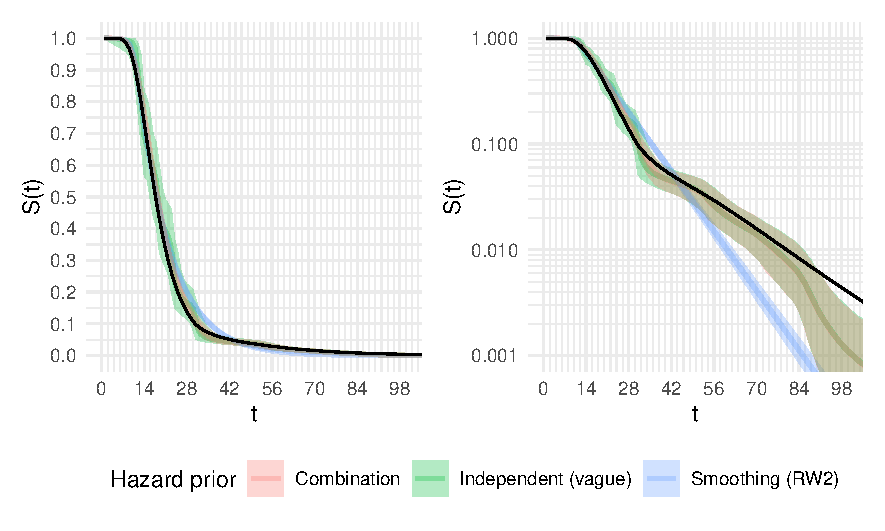
\includegraphics{cis-perfect-testing/survival-results}
  \caption[Comparison of survival function estimates under different priors]{Comparison of the posterior estimate of the survival distribution (pointwise median and 95\% CrI) when using different priors on the hazard. Results using each of the three different priors discussed in \cref{perf-test:sec:parameters-priors} are shown. y-axis has either natural (left) or log (right) scale. I show only the first 100 days of the distribution for readability. \label{perf-test:fig:survival-results}}
\end{figure}

\begin{figure}
  \centering 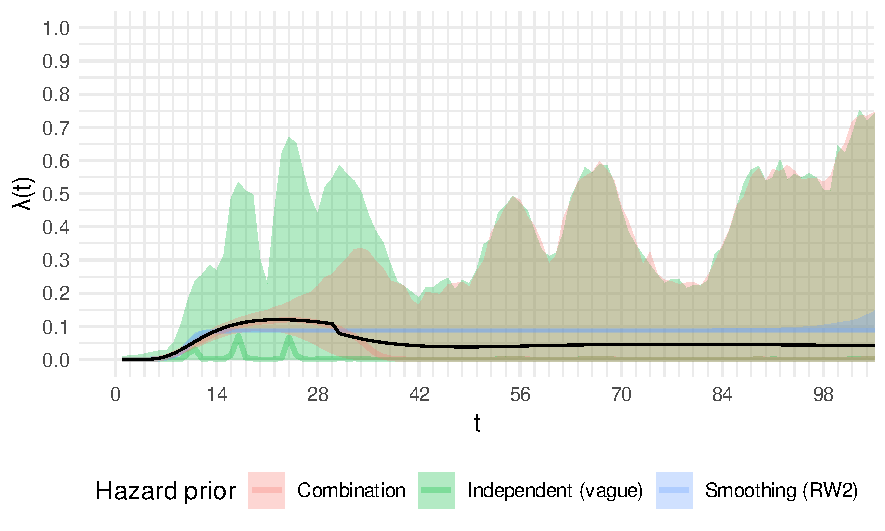
\includegraphics{cis-perfect-testing/hazard-results}
  \caption[Comparison of hazard estimates under different priors]{Comparison of the posterior estimate of the hazard (pointwise median and 95\% CrI) when using different priors on the hazard. Results using each of the three different priors discussed in \cref{perf-test:sec:parameters-priors} are shown. \label{perf-test:fig:hazard-results}}
\end{figure}

\section{Discussion} \label{perf-test:sec:discussion}

This chapter shows that the model I propose can recover the true survival function well.
However, the problem becomes substantially harder if false negatives are present, as we shall see in the next chapter.
Unfortunately, false negatives do occur in the CIS data.

Reasonable choices of the prior for the hazard are vague (although not flat) or informative.
A smoothing prior performed poorly, although that may be influenced by the choice of hyperparameters.
Reducing the amount of smoothing or type of smoothing may help.
More flexible smoothers, such as a Gaussian Process for additional flexibility and smoothing and different timescales~\autocite{saulGaussian}.

Various extensions could be worth exploring.
Most importantly, including covariates (\eg age, immunity from vaccination and/or previous infection, or variant).
Immunity in particular affects the duration substantially, although age and variant may also make a contribution~\autocite{hakkiOnset,russellWithinhost}.
Covariates can be included with a variety of models, the simplest being a proportional hazards model.
A major challenge here is that the calculation of $p_t$ is greatly complicated because it is no longer linear in the survival function.

The prior would likely be more important if the number of detected infections was smaller.
Therefore, exploring its impact could be important for future surveys.
A particular application would be estimation in the early stages of an epidemic of a novel pathogen.
Here, little would be known about the pathogen, but gathering information with robust estimates of uncertainty is important to inform the response.

I have assumed a prior of constant incidence and that incidence is independent between individuals.
Prevalence in the CIS data was approximately constant over the period of interest (see \cref{E-biology-data:sec:positivity-results}).
A sensitivity analysis, where an epidemic in exponential growth or decline was simulated (not shown), showed minimal impact on survival estimates.
An incorrect assumption of constant incidence can lead to biased estimates~\autocite{degruttolaAnalysis}.
Therefore, the assumption could be important in other contexts, especially if the incidence is changing rapidly.

I have developed a flexible simulation and inference framework for this type of analysis.
This framework could be used to simulate alternate study designs.
The design of CIS was created on a very short timescale in March 2020, in response to the pandemic's rapid spread.
Therefore, it is likely that there are more efficient designs.
These could be more cost-effective.
Improved cost-effectiveness could allow more rapid response to potential pandemics because the threshold for policymakers to approve the study would be lower.
A long-term, preparatory effort to develop a more efficient design in preparation for a future pandemic would be worthwhile.

Other useful preparatory work would be developing reasonable priors.
These could be based on seasonal viruses that are of the same family as those likely to cause future pandemics.
For example, seasonal influenzas and coronaviruses.
These would allow analyses such as those performed in these chapters to be performed more rapidly in a future pandemic scenario.

\section{Conclusion} \label{perf-test:sec:conclusion}
This chapter has shown the feasibility of estimating the survival function from a study with a CIS-like testing schedule.
While the infrequent testing schedule is not ideal, appropriate modelling can recover the true survival function well.

\ifSubfilesClassLoaded{
  \listoftodos
}{}
\end{document}